\documentclass{beamer-control}
\usepackage{beamer-control-singlefile}
\INCLUDEONLY{Determining the Transfer Function}
\begin{document}
\CONCEPT{Determining the Transfer Function}

\begin{SUMMARY}
\begin{itemize}
\item Transmission of Exponential Signals
\item Transfer Functions for Linear Differential Equations
\begin{itemize}
\item Definition of poles and zeros
\end{itemize}
\item State Space Realisations of Transfer Functions
\end{itemize}
\vfill References:
\begin{itemize}
\item \astrom{§9.2}
\end{itemize}
\end{SUMMARY}

\SUBCONCEPT{Transmission of Exponential Signals}

\begin{frame}{The exponential signal}
\begin{itemize}
\item Define the \alert{exponential signal} $\ee^{st}$ where $s=\sigma+\ii\ww$
\end{itemize}
\begin{align}
\ee^{(\sigma+\ii\ww)t} = \ee^{\sigma t}\ee^{\ii\ww t} = \ee^{\alpha t}\left( \cos\ww t + \ii \sin \ww t \right)
\end{align}
\begin{itemize}
\item This signal allows use to representing growth/decay and/or oscillation
\end{itemize}
\end{frame}

\begin{frame}
\frametitle{Exponential signals}
\centering
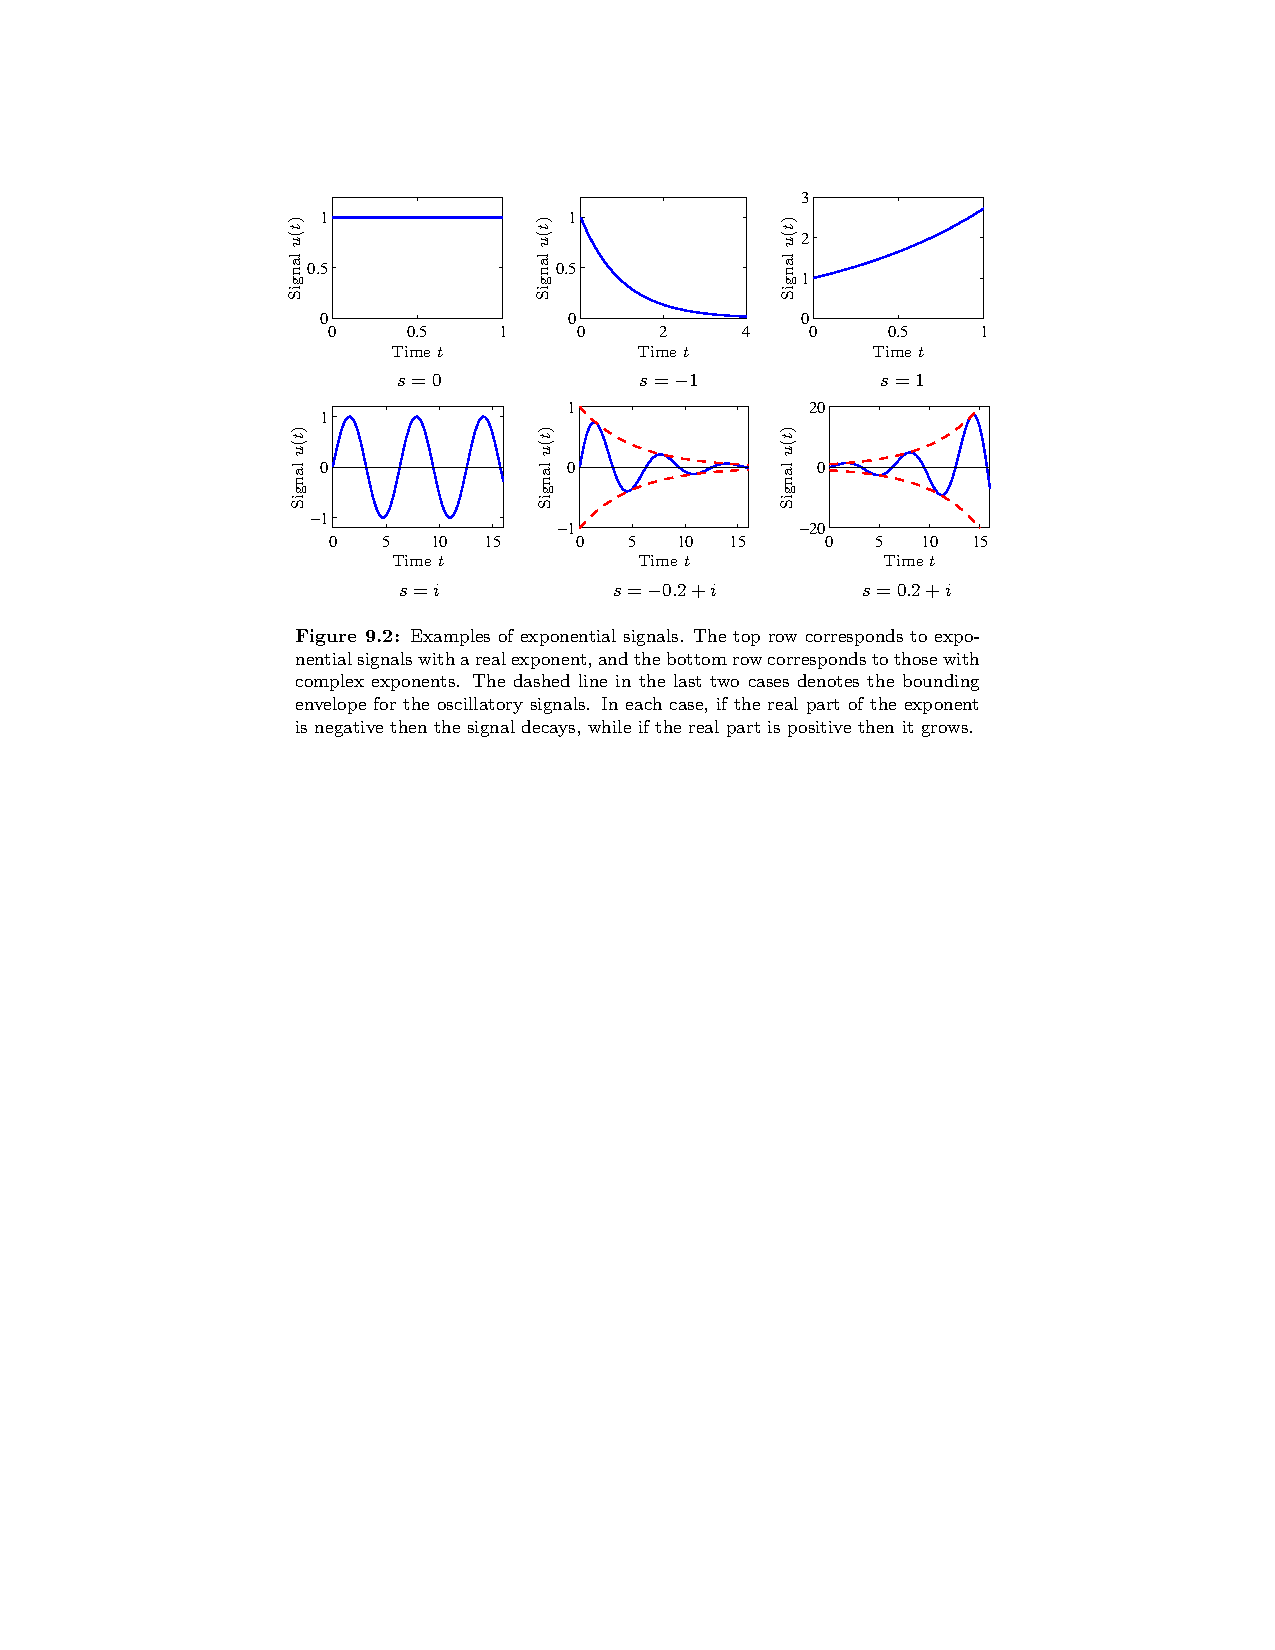
\includegraphics[width=0.8\linewidth]{figure9.2}
\end{frame}

\begin{frame}
\frametitle{Input to output}
\begin{itemize}
\item
With state space system with input $u(t)=\ee^{st}$ we can derive the state $x(t)$
\item
With the state $x(t)$ we can derive the output $y(t)$
\item
$y(t)$ consists of: (transient response terms) + \\\hfill (pure exponential response $y_p(t)$)
\item
The transfer function captures steady state output, so we define:
\end{itemize}
\begin{align}
y_p(t) &= G(s) \ee^{st} \,, \\
G(s) &= C(sI-A)\Inv B + D
\end{align}
Note: $s=\lambda_j(A)$ are special values of $s$ --- important later!
\end{frame}


\begin{frame}
\frametitle{Damped Oscillator \AMref{Example 9.1}}
We've looked previously at the damped oscillator (aka mass-spring-damper in mecheng):
\begin{align}
\Deriv{x}{t} &= \Matr{0 & \ww_0\\ -\ww_0 & -2\zz\ww_0}x+\Matr{0\\ k\ww_0}u & y&= \Matr{1 & 0} x
\end{align}
With $\zeta>0$ and input $u(t)=\ee^{s t}$:
\begin{align}
G_{yu}(s) &= C(sI-A)\Inv B = \cdots = \frac{k \ww_0^2}{s^2 + 2\zz\ww_0 s + \ww_0^2}
\end{align}
\end{frame}


\begin{frame}
\frametitle{Damped Oscillator \AMref{Example 9.1}}
For a step input, $s=0$ ($\therefore~ u(t) = \Exp{0 t} = 1$):
\begin{align}
G_{yu}(0) = \left.\frac{k \ww_0^2}{s^2 + 2\zz\ww_0 s + \ww_0^2}\right|_{s=0} = k
\end{align}
For a sinusoidal input, $u=\sin\ww t$ and there is all sorts of elegant maths which we can boil down to:
\begin{align}
y &= M \sin(\ww t + \theta) \,, \\
M &= \abs\left( G(\ii\ww) \right) \\
\theta &= \arg\left( G(\ii\ww) \right)
\end{align}
You can do this analytically, and it is very fun, but generally not needed
\end{frame}


\SUBCONCEPT{Transfer Functions for Linear Differential Equations}

\begin{frame}{Linear Differential Equations}
Consider generalised linear system with input $u$ and output $y$:
\begin{align}
\Deriv{^n y}{t^n} + a_1 \Deriv{^{n-1} y}{t^{n-1}} + \cdots + a_n y = 
b_0 \Deriv{^m u}{t^m} + b_1 \Deriv{^{m-1} u}{t^{m-1}} + \cdots + b_m u
\end{align}
As $u(t)=\Exp{s t}$ gives $y(t)=y_0 \Exp{s t}$:
\begin{math}
\Deriv{^k u}{t^k} = s^k \Exp{s t}
\end{math}
and
\begin{math}
\Deriv{^k y}{t^k} = y_0 s^k \Exp{s t} 
\end{math}
\begin{multline}
y_0 s^n \Exp{s t} + a_1 y_0 s^{n-1} \Exp{s t} + \cdots + a_n y_0 \Exp{s t} = \\
b_0 s^m \Exp{s t} + b_1 s^{m-1} \Exp{s t} + \cdots + b_m \Exp{s t}
\end{multline}
\begin{align}
a(s) y_0 \Exp{s t} &= b(s) \Exp{s t} & y(t) &= \frac{b(s)}{a(s)}\Exp{s t}
\end{align}
\end{frame}

\begin{frame}
\frametitle{Poles and zeros}
\begin{align}
G(s) = \frac{b(s)}{a(s)} = \frac
  { b_0 s^m  + b_1 s^{m-1}  + \cdots + b_m  }
  { s^n + a_1 s^{n-1} + \cdots + a_n  }
\end{align}
Define:
\begin{itemize}
\item Zeros of $G(s)$: the roots of the polynomial $b(s)$
\item Poles of $G(s)$: the roots of the polynomial $a(s)$
\end{itemize}
These poles and zeros define important properties of the transfer function

\bigskip
\begin{uncoverenv}<2->
BTW: Poles of $G(s)$ = $\lambda_j(A)$, the eigenvalues of $A$ !
\end{uncoverenv}
\end{frame}

\begin{frame}
\frametitle{Common LTI systems}
\framesubtitle{Note the time delay}

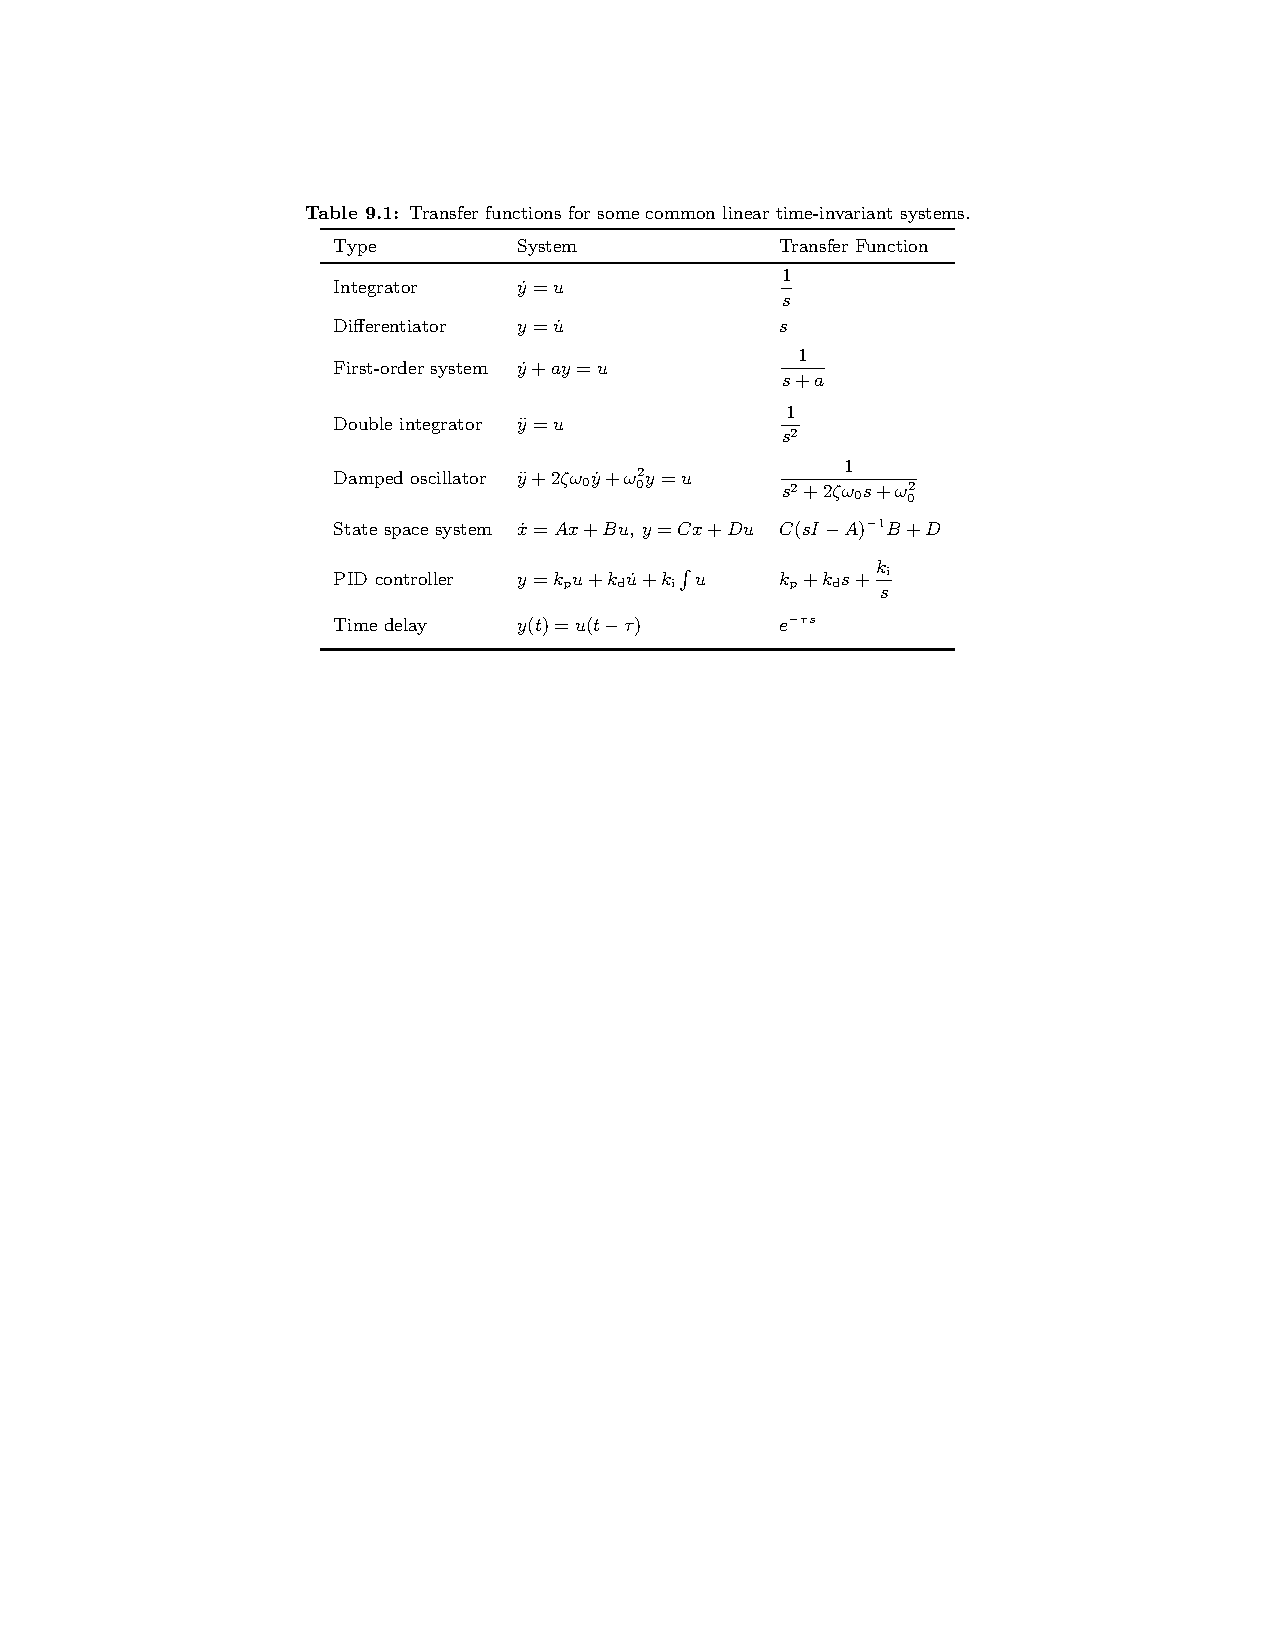
\includegraphics[height=0.8\textheight]{table9.1}


\end{frame}


\SUBCONCEPT{State Space Realisations of Transfer Functions}

\begin{frame}
\frametitle{State space vs Transfer function}
\begin{align}
\dot x &= A x + B u \,, & 
y &= Cx + Du \,, &
G(s) &= C(sI-A)\Inv B+D
\end{align}
\begin{itemize}
\item
We have seen previously that $A$, $B$, $C$, $D$ can be transformed and are not unique for a given dynamical system
\item
$G(s)$, however, is unique
\item
Textbook \AMref{Example 9.7} shows a case of \alert{pole/zero cancellation} where the transfer function ended up simpler than the state space model
\item
The \emph{minimal realisation} (\texttt{minreal()} in Matlab) is the lowest-order version of the system
\end{itemize}
\end{frame}


\SUMMARYFRAME
\FINALE

\end{document}
